\chapter{Support Vector Machines}\label{ch-13}

Le \textbf{Support Vector Machines} (SVM) sono la risposta alla domanda
lasciata aperta dalla SLT
(\href{12\%20-\%20Statistical\%20Learning\%20Theory\%20e\%20VC-dimension}{12
- Statistical Learning Theory e VC-dimension}): è possibile fissare
l'errore di training e minimizzare \textbf{automaticamente} la
VC-confidence? L'SVM è ancora una macchina lineare (una LTU), ma sceglie
tra tutti gli iperpiani separatori quello che \textbf{massimizza il
margine}, e questo equivale a controllare la VC-dimension. La lezione
procede in quattro passi: SVM lineare \emph{hard margin}, SVM \emph{soft
margin} per dati non separabili, \textbf{kernel} per problemi non
lineari, e infine SVM per la \textbf{regressione}.

\begin{boxnote}{Notazione (da Haykin, cap. 6)}

\(N\) è il numero di esempi (prima \(l\)), con indici \(i\) e \(j\) per
i pattern; \(m\) è la dimensione del vettore di input (prima \(n\)); si
usa \(b\) invece di \(w_0\) per il bias. Le parti segnate con * nelle
slide sono utili per completezza ma non indispensabili per usare il
modello (e per un orale standard): in particolare i dettagli della
risoluzione con i moltiplicatori di Lagrange.

\end{boxnote}

\section{Parte I --- SVM per la classificazione
binaria}\label{parte-i-svm-per-la-classificazione-binaria}

Una SVM è:

\begin{itemize}
\tightlist
\item
  una \textbf{macchina lineare} (come la LTU o il Perceptron);
\item
  che \textbf{massimizza il margine di separazione};
\item
  e realizza una \textbf{Structural Risk Minimization}.
\end{itemize}

Inizialmente (SVM \emph{hard margin}) si assume che il problema sia
\textbf{linearmente separabile} e che \textbf{non ci siano errori} nei
dati.

\begin{figure}[htbp]
\centering
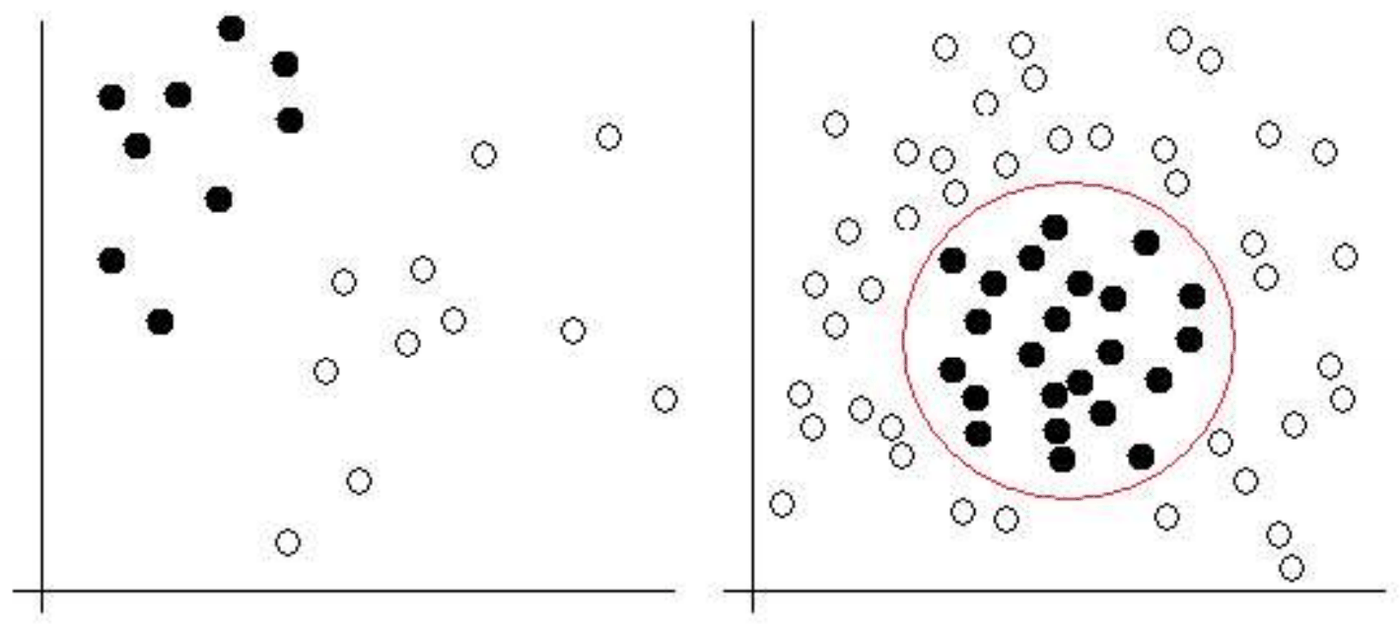
\includegraphics[width=0.71\linewidth,height=0.42\textheight,keepaspectratio]{images/13-svm_separabili.png}
\caption{Pattern linearmente separabili (sinistra) e non linearmente separabili
(destra).}
\end{figure}

\subsection{L'iperpiano separatore}\label{liperpiano-separatore}

Dato il training set \(T = \{(\mathbf{x}_i, d_i)\}_{i=1}^{N}\), si cerca
un iperpiano \(\mathbf{w}^T\mathbf{x} + b = 0\) che separi gli esempi:
\[
\mathbf{w}^T\mathbf{x}_i + b \ge 0 \;\text{ se } d_i = +1, \qquad \mathbf{w}^T\mathbf{x}_i + b < 0 \;\text{ se } d_i = -1.
\] \(g(\mathbf{x}) = \mathbf{w}^T\mathbf{x} + b\) è la \textbf{funzione
discriminante} e \(h(\mathbf{x}) = \operatorname{sign}(g(\mathbf{x}))\)
è l'\textbf{ipotesi}.

\subsection{Il margine di separazione}\label{il-margine-di-separazione}

\begin{boxdefinition}{Margine di separazione}

Se l'iperpiano è alla stessa distanza dal più vicino esempio positivo e
dal più vicino negativo, il \textbf{margine di separazione} \(\rho\) è
il doppio della distanza tra l'iperpiano e il punto più vicino. Lo si
può pensare come una \textbf{``zona di sicurezza''} attorno al confine.

\end{boxdefinition}

\begin{figure}[htbp]
\centering
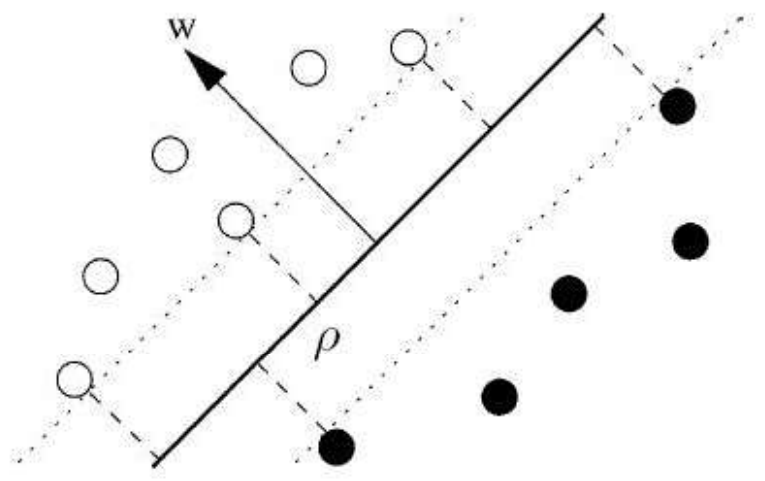
\includegraphics[width=0.43\linewidth,height=0.42\textheight,keepaspectratio]{images/13-svm_margine.png}
\caption{Il margine di separazione \(\rho\).}
\end{figure}

Non tutti gli iperpiani che risolvono il problema sono uguali: al
variare dell'iperpiano separatore varia anche il margine.

\begin{figure}[htbp]
\centering
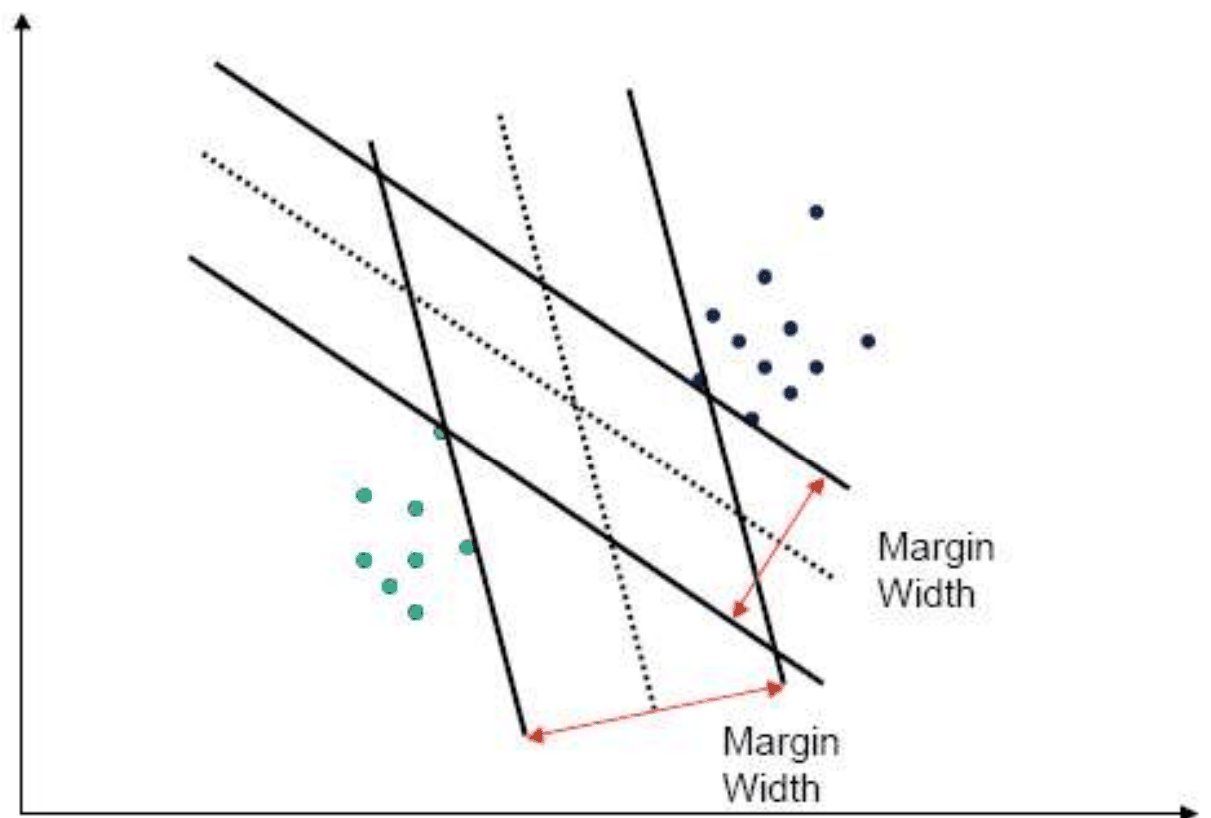
\includegraphics[width=0.60\linewidth,height=0.42\textheight,keepaspectratio]{images/13-svm_margini-diversi.png}
\caption{Iperpiani separatori diversi hanno margini diversi.}
\end{figure}

\begin{boxdefinition}{Iperpiano ottimo}

L'\textbf{iperpiano ottimo} \(\mathbf{w}_o^T\mathbf{x} + b_o = 0\)
(``o'' sta per \emph{optimal}) è quello che \textbf{massimizza il
margine} \(\rho\). Vedremo che \(\rho = \dfrac{2}{\|\mathbf{w}\|}\),
quindi \[
\text{massimizzare } \rho \iff \text{minimizzare } \|\mathbf{w}\|.
\]

\end{boxdefinition}

\subsection{Rappresentazione canonica e support
vector}\label{rappresentazione-canonica-e-support-vector}

Per la \textbf{libertà di scala} (moltiplicando \(\mathbf{w}\) e \(b\)
per una costante l'iperpiano non cambia) possiamo riscalare
\(\mathbf{w}\) e \(b\) in modo che i punti più vicini all'iperpiano
soddisfino \(|g(\mathbf{x}_i)| = |\mathbf{w}^T\mathbf{x}_i + b| = 1\).
Allora: \[
\mathbf{w}^T\mathbf{x}_i + b \ge 1 \;\text{ se } d_i = +1, \qquad \mathbf{w}^T\mathbf{x}_i + b \le -1 \;\text{ se } d_i = -1,
\] cioè, in forma compatta: \[
d_i(\mathbf{w}^T\mathbf{x}_i + b) \ge 1 \qquad \forall i = 1,\dots,N.
\]

\begin{boxdefinition}{Support vector}

Un \textbf{support vector} \(\mathbf{x}^{(s)}\) soddisfa il vincolo
\textbf{con l'uguaglianza}:
\(d^{(s)}(\mathbf{w}^T\mathbf{x}^{(s)} + b) = 1\). I support vector sono
i punti \textbf{più vicini} all'iperpiano, quelli che stanno sul bordo
del margine.

\end{boxdefinition}

\begin{figure}[htbp]
\centering
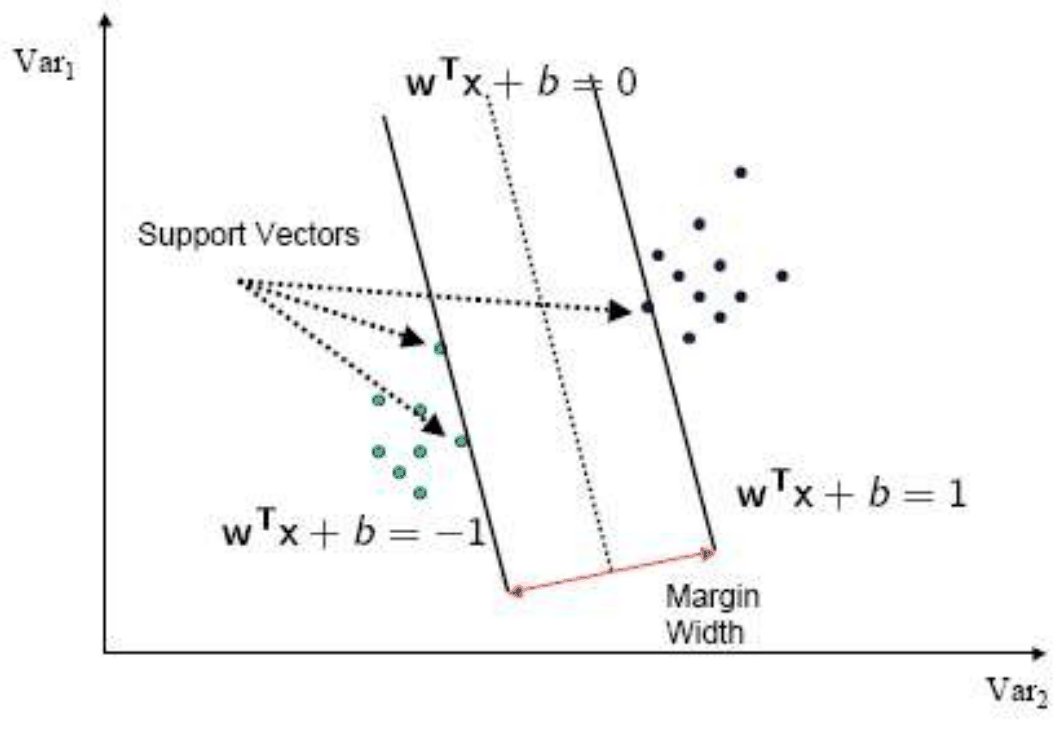
\includegraphics[width=0.60\linewidth,height=0.42\textheight,keepaspectratio]{images/13-svm_support-vectors.png}
\caption{I support vector giacciono sulle rette
\(\mathbf{w}^T\mathbf{x} + b = \pm 1\).}
\end{figure}

\subsection{Calcolo del margine}\label{calcolo-del-margine}

\textbf{Distanza di un punto dall'iperpiano.} Sia \(r\) la distanza tra
\(\mathbf{x}\) e l'iperpiano ottimo. Poiché \(\mathbf{w}_o\) è
ortogonale all'iperpiano, possiamo scrivere \[
\mathbf{x} = \mathbf{x}_p + r\,\frac{\mathbf{w}_o}{\|\mathbf{w}_o\|},
\] dove \(\mathbf{x}_p\) è la proiezione di \(\mathbf{x}\)
sull'iperpiano.

\begin{figure}[htbp]
\centering
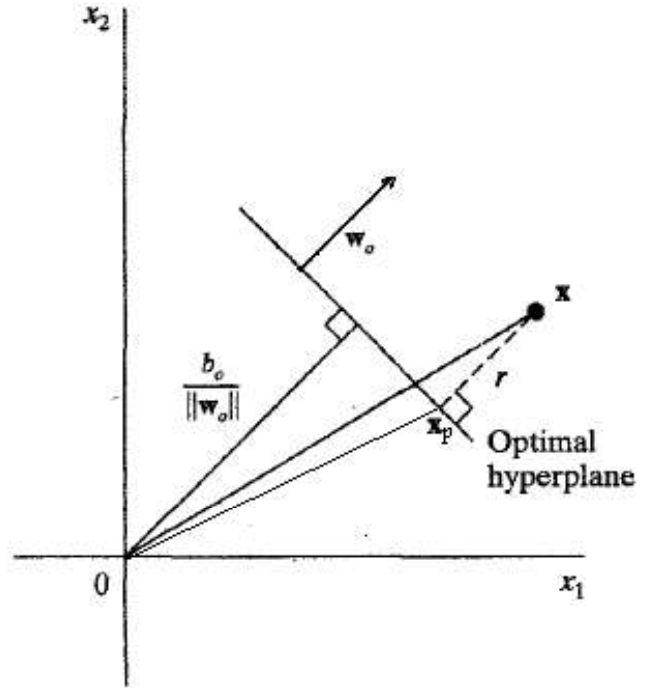
\includegraphics[width=0.43\linewidth,height=0.42\textheight,keepaspectratio]{images/13-svm_distanza.png}
\caption{Distanza \(r\) tra un punto \(\mathbf{x}\) e l'iperpiano ottimo.}
\end{figure}

Valutando \(g(\mathbf{x}) = \mathbf{w}_o^T\mathbf{x} + b_o\): \[
g(\mathbf{x}) = \mathbf{w}_o^T\mathbf{x}_p + b_o + r\,\mathbf{w}_o^T\frac{\mathbf{w}_o}{\|\mathbf{w}_o\|} = \underbrace{g(\mathbf{x}_p)}_{=0} + r\,\frac{\|\mathbf{w}_o\|^2}{\|\mathbf{w}_o\|} = r\,\|\mathbf{w}_o\|,
\] perché \(\mathbf{x}_p\) sta sull'iperpiano. Quindi \[
r = \frac{g(\mathbf{x})}{\|\mathbf{w}_o\|}.
\]

\textbf{Margine.} Per un support vector positivo
\(g(\mathbf{x}^{(s)}) = 1\), quindi la sua distanza dall'iperpiano è
\(r = \frac{1}{\|\mathbf{w}_o\|} = \frac{\rho}{2}\). Da cui: \[
\rho = \frac{2}{\|\mathbf{w}_o\|}.
\] L'iperpiano ottimo massimizza \(\rho\), cioè \textbf{minimizza
\(\|\mathbf{w}\|\)}.

\subsection{Il problema di ottimizzazione quadratica (hard
margin)}\label{il-problema-di-ottimizzazione-quadratica-hard-margin}

La derivazione formale richiede tecniche di \textbf{ottimizzazione
vincolata} (assunte note, ad esempio dal corso CM); la programmazione
quadratica si considera risolta da pacchetti esistenti. Qui interessa
capire come è formulato il problema, la relazione tra support vector e
moltiplicatori \(\alpha\), e il risultato finale per \(\mathbf{w}_o\).

\begin{boxdefinition}{Problema primale --- SVM hard margin}

Dato \(T = \{(\mathbf{x}_i, d_i)\}_{i=1}^N\), trovare \(\mathbf{w}\) e
\(b\) che minimizzano \[
\Psi(\mathbf{w}) = \frac{1}{2}\mathbf{w}^T\mathbf{w} \qquad (\text{cioè } \min \|\mathbf{w}\|)
\] soggetto ai vincoli (zero errori di classificazione) \[
d_i(\mathbf{w}^T\mathbf{x}_i + b) \ge 1 \qquad \forall i = 1,\dots,N.
\]

\end{boxdefinition}

\begin{itemize}
\tightlist
\item
  La funzione obiettivo è \textbf{quadratica e convessa} in
  \(\mathbf{w}\).
\item
  I vincoli sono \textbf{lineari} in \(\mathbf{w}\).
\item
  Risolvere questo problema scala con la dimensione dello spazio di
  input \(m\) (il costo effettivo dipende comunque dall'algoritmo del
  risolutore).
\end{itemize}

\subsubsection{Soluzione con i moltiplicatori di
Lagrange*}\label{soluzione-con-i-moltiplicatori-di-lagrange}

Si costruisce la \textbf{lagrangiana}: \[
J(\mathbf{w}, b, \boldsymbol{\alpha}) = \frac{1}{2}\mathbf{w}^T\mathbf{w} - \sum_{i=1}^{N}\alpha_i\big(d_i(\mathbf{w}^T\mathbf{x}_i + b) - 1\big),
\] con \(\alpha_i \ge 0\) i \textbf{moltiplicatori di Lagrange}, uno per
ogni vincolo del primale. \(J\) va \textbf{minimizzata rispetto a
\(\mathbf{w}\) e \(b\)} e \textbf{massimizzata rispetto ad
\(\boldsymbol{\alpha}\)}: la soluzione è un \textbf{punto di sella} di
\(J\).

Condizioni di ottimalità: \[
\frac{\partial J}{\partial \mathbf{w}} = 0 \;\Rightarrow\; \mathbf{w} = \sum_{i=1}^{N}\alpha_i d_i\mathbf{x}_i, \qquad \frac{\partial J}{\partial b} = 0 \;\Rightarrow\; \sum_{i=1}^{N}\alpha_i d_i = 0.
\]

\textbf{Condizioni di Kuhn-Tucker.} Nel punto di sella vale \[
\alpha_i\big(d_i(\mathbf{w}^T\mathbf{x}_i + b) - 1\big) = 0 \qquad \forall i.
\] Quindi:

\begin{itemize}
\tightlist
\item
  se \(\alpha_i > 0\), allora \(d_i(\mathbf{w}^T\mathbf{x}_i + b) = 1\):
  \(\mathbf{x}_i\) è un \textbf{support vector};
\item
  se \(\mathbf{x}_i\) non è un support vector, allora \(\alpha_i = 0\).
\end{itemize}

\begin{boxtip}{L'iperpiano dipende solo dai support vector}

\(\mathbf{w}_o = \sum_{i=1}^{N_s}\alpha_{o,i}\,d_i\,\mathbf{x}_i\): la
somma si restringe agli \(N_s\) support vector. \textbf{L'iperpiano
dipende solo dai support vector!} Tutti gli altri punti potrebbero
essere rimossi senza cambiare la soluzione.

\end{boxtip}

\subsubsection{Il problema duale*}\label{il-problema-duale}

Sostituendo le condizioni di ottimalità in \(J\) si ottiene il
\textbf{problema duale}, in cui compaiono solo i moltiplicatori:

\begin{boxdefinition}{Problema duale --- SVM hard margin}

Trovare \(\{\alpha_i\}_{i=1}^N\) che massimizzano \[
Q(\boldsymbol{\alpha}) = \sum_{i=1}^{N}\alpha_i - \frac{1}{2}\sum_{i=1}^{N}\sum_{j=1}^{N}\alpha_i\alpha_j d_i d_j\,\mathbf{x}_i^T\mathbf{x}_j
\] soggetto a \(\alpha_i \ge 0\) per ogni \(i\) e
\(\sum_{i=1}^{N}\alpha_i d_i = 0\).

\end{boxdefinition}

Gli \(\alpha\) si trovano risolvendo il problema di
\textbf{programmazione quadratica} (QP) o con approcci più recenti ed
efficienti (ad esempio \textbf{SMO}, \emph{Sequential Minimal
Optimization}). Il duale scala con il \textbf{numero di esempi \(N\)},
meno con la dimensione dello spazio. Si noti che i dati compaiono
\textbf{solo tramite prodotti scalari} \(\mathbf{x}_i^T\mathbf{x}_j\):
sarà la chiave dei kernel.

\subsubsection{\texorpdfstring{Ottenere \(\mathbf{w}_o\) e
\(b_o\)}{Ottenere \textbackslash mathbf\{w\}\_o e b\_o}}\label{ottenere-mathbfw_o-e-b_o}

\begin{enumerate}
\def\labelenumi{\arabic{enumi}.}
\tightlist
\item
  Risolvere il duale ottenendo \(\{\alpha_{o,i}\}\).
\item
  Calcolare \(\mathbf{w}_o = \sum_{i=1}^N\alpha_{o,i}d_i\mathbf{x}_i\).
\item
  Calcolare \(b_o = 1 - \mathbf{w}_o^T\mathbf{x}^{(s)}\) per un support
  vector positivo \(\mathbf{x}^{(s)}\), cioè
  \(b_o = 1 - \sum_{i=1}^N\alpha_{o,i}d_i\,\mathbf{x}_i^T\mathbf{x}^{(s)}\).
\end{enumerate}

\subsection{Come si usa}\label{come-si-usa}

Non serve conoscere esplicitamente \(\mathbf{w}_o\): bastano i
moltiplicatori (dal duale) e il bias. La superficie di decisione è \[
\mathbf{w}_o^T\mathbf{x} + b_o = 0 \iff \sum_{i=1}^N\alpha_{o,i}\,d_i\,\underbrace{\mathbf{x}_i^T\mathbf{x}}_{\text{prodotto scalare}} + b_o = 0.
\] Dato un pattern \(\mathbf{x}\): (1) calcolare
\(g(\mathbf{x}) = \sum_{i=1}^N\alpha_{o,i}d_i\,\mathbf{x}_i^T\mathbf{x} + b_o\);
(2) classificare con il segno di \(g(\mathbf{x})\). La somma si può
restringere agli \(N_s\) support vector.

\subsection{Perché migliora la
generalizzazione?}\label{perchuxe9-migliora-la-generalizzazione}

Su problemi linearmente separabili abbiamo \textbf{fissato l'errore di
training} (a zero). Minimizzare la norma di \(\mathbf{w}\) equivale
allora a \textbf{minimizzare la VC-dimension}, e quindi il termine di
capacità (VC-confidence) \(\varepsilon\) in \[
R[h] \le R_{emp}[h] + \varepsilon(VC, N, \delta).
\]

\begin{boxtheorem}{Teorema di Vapnik}

Sia \(D\) il diametro della più piccola sfera che contiene i dati
\(\mathbf{x}_1,\dots,\mathbf{x}_N\). Per la classe degli iperpiani
separatori \(\mathbf{w}^T\mathbf{x} + b = 0\) con margine \(\rho\), la
VC-dimension è limitata da \[
VC \le \min\left(\left\lceil\frac{D^2}{\rho^2}\right\rceil, m_0\right) + 1.
\]

\end{boxtheorem}

Poiché \(\frac{D^2}{\rho^2} \propto \text{Raggio}^2\,\|\mathbf{w}\|^2\),
la VC-dim può essere \textbf{minore di \(m_0 + 1\)} (quella degli
iperpiani generici) restringendo la ricerca agli iperpiani
``regolarizzati'' con margine massimo. \textbf{Più il margine è grande,
più la VC-dim è piccola}, indipendentemente dalla dimensione dello
spazio.

\subsection{Perché è un approccio
elegante}\label{perchuxe9-uxe8-un-approccio-elegante}

Per dati linearmente separabili ci sono molte soluzioni; Vapnik propone
l'\textbf{iperpiano separatore ottimo} a margine massimo, che fornisce:

\begin{itemize}
\tightlist
\item
  una \textbf{soluzione unica} (a differenza dell'algoritmo iterativo
  del Perceptron) con \textbf{zero errori} (a differenza dell'LMS) per
  il classificatore binario;
\item
  un'\textbf{SRM automatizzata}, che minimizza la VC-confidence
  (massimizzando il margine) direttamente all'interno del processo di
  ottimizzazione, \textbf{senza iperparametri} nel caso separabile;
\item
  l'uso di risolutori di \textbf{programmazione quadratica vincolata}
  (anziché la discesa del gradiente), con una bella forma duale che
  mostra i support vector e i prodotti scalari tra pattern;
\item
  una soluzione concentrata su dati di training
  \textbf{``selezionati''}, i support vector: pregio, perché non dipende
  dai punti lontani dal confine; difetto, perché si spera che i punti
  sul confine non siano i più rumorosi.
\end{itemize}

Ma cosa fare con dati \textbf{rumorosi} o \textbf{non linearmente
separabili}?

\section{SVM soft margin: ammettere
errori}\label{svm-soft-margin-ammettere-errori}

Se almeno un punto viola la condizione di separazione esatta
\(d_i(\mathbf{w}^T\mathbf{x}_i + b) \ge 1\), si passa al \textbf{soft
margin}.

\begin{figure}[htbp]
\centering
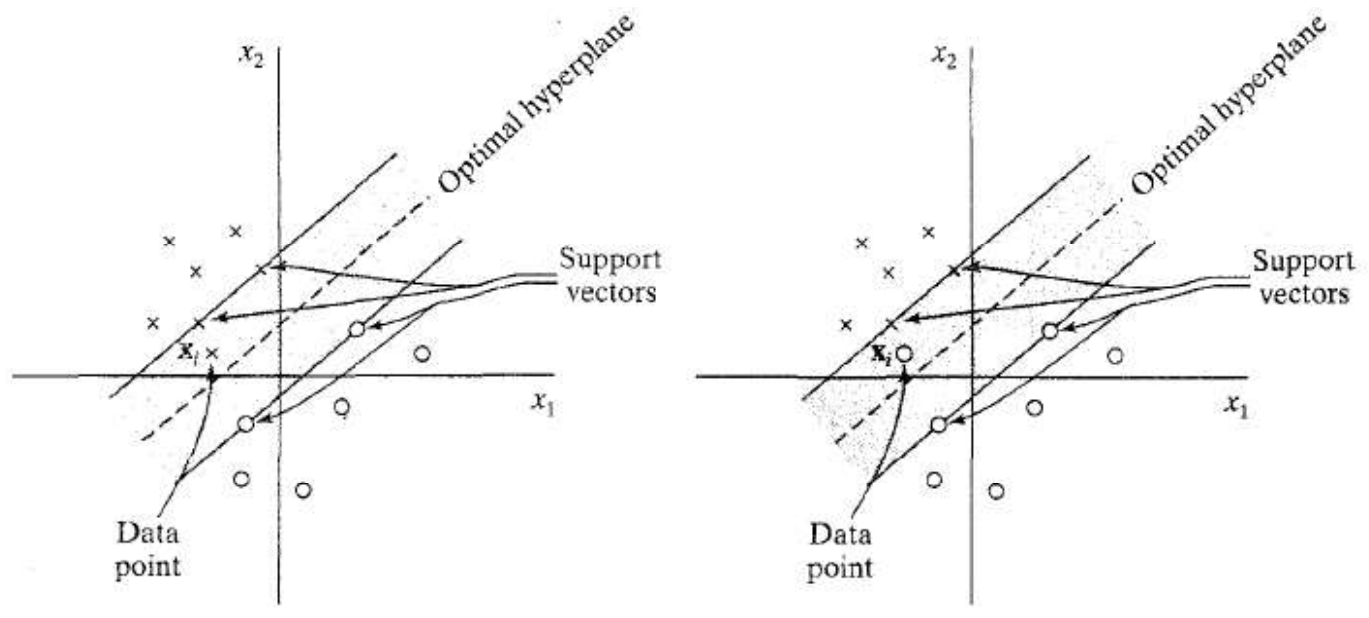
\includegraphics[width=0.71\linewidth,height=0.42\textheight,keepaspectratio]{images/13-svm_soft-margin.png}
\caption{Pattern che violano il margine, senza (sinistra) e con (destra) errore
di classificazione.}
\end{figure}

\begin{boxtip}{Il vantaggio del soft margin}

Ammettere punti dentro il margine permette di avere un \textbf{margine
più ampio}: si ottiene tolleranza al rumore e un modello più semplice.
(Esercizio: trovare il margine delle figure senza ammettere punti al suo
interno.)

\end{boxtip}

\subsection{Variabili slack}\label{variabili-slack}

Si introducono variabili non negative \(\xi_i \ge 0\), dette
\textbf{variabili slack}, e i vincoli diventano \[
d_i(\mathbf{w}^T\mathbf{x}_i + b) \ge 1 - \xi_i \qquad \forall i.
\] - \(\xi_i = 0\): il punto è fuori dal margine o sul bordo; -
\(0 < \xi_i \le 1\): il punto è dentro il margine ma classificato
correttamente; - \(\xi_i > 1\): il punto è classificato male.

Un support vector soddisfa ora
\(d_i(\mathbf{w}^T\mathbf{x}_i + b) = 1 - \xi_i\).

\begin{figure}[htbp]
\centering
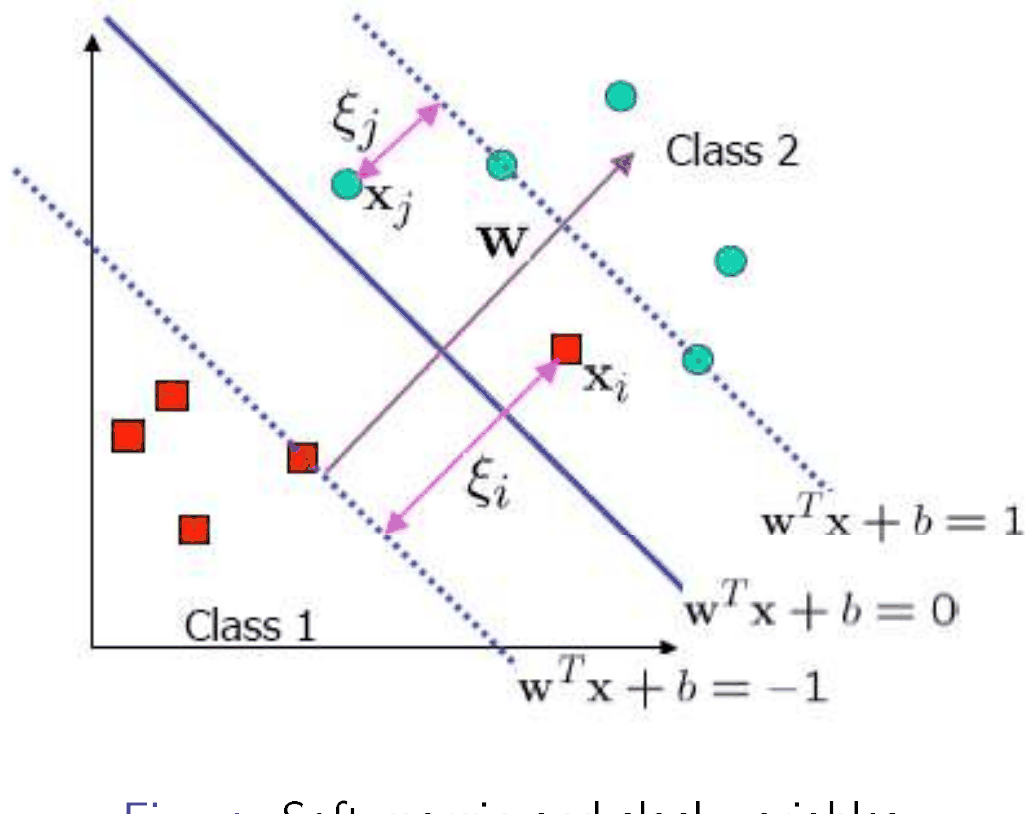
\includegraphics[width=0.54\linewidth,height=0.42\textheight,keepaspectratio]{images/13-svm_slack.png}
\caption{Soft margin e variabili slack.}
\end{figure}

Attenzione: il \textbf{teorema di Vapnik non vale più} (l'hard margin
non ammette punti nel margine).

\subsection{Il problema primale soft
margin}\label{il-problema-primale-soft-margin}

\begin{boxdefinition}{Problema primale --- SVM soft margin}

Trovare \(\mathbf{w}\) e \(b\) che minimizzano \[
\Psi(\mathbf{w}, \boldsymbol{\xi}) = \frac{1}{2}\mathbf{w}^T\mathbf{w} + C\sum_{i=1}^{N}\xi_i
\] soggetto a \(d_i(\mathbf{w}^T\mathbf{x}_i + b) \ge 1 - \xi_i\) e
\(\xi_i \ge 0\) per ogni \(i\).

\end{boxdefinition}

\(C\) è un \textbf{iperparametro di regolarizzazione} (si perde la SRM
completamente automatica!): regola il compromesso tra minimizzazione del
rischio empirico e minimizzazione del termine di capacità
(VC-confidence).

\begin{itemize}
\tightlist
\item
  \textbf{\(C\) basso}: molti errori di training ammessi → possibile
  \textbf{underfitting}.
\item
  \textbf{\(C\) alto}: nessun errore ammesso → margine più piccolo →
  possibile \textbf{overfitting}.
\end{itemize}

(Per \(C \to \infty\) si ritrova l'hard margin.)

\subsection{Il duale soft margin*}\label{il-duale-soft-margin}

\begin{boxdefinition}{Problema duale --- SVM soft margin}

Trovare \(\{\alpha_i\}\) che massimizzano \[
Q(\boldsymbol{\alpha}) = \sum_{i=1}^{N}\alpha_i - \frac{1}{2}\sum_{i=1}^{N}\sum_{j=1}^{N}\alpha_i\alpha_j d_i d_j\,\mathbf{x}_i^T\mathbf{x}_j
\] soggetto a \(\sum_{i=1}^{N}\alpha_i d_i = 0\) e
\(0 \le \alpha_i \le C\) per ogni \(i\).

\end{boxdefinition}

È \textbf{identico} al caso hard margin, tranne il vincolo superiore
\(\alpha_i \le C\). Le condizioni di Kuhn-Tucker diventano \[
\alpha_i\big(d_i(\mathbf{w}^T\mathbf{x}_i + b) + \xi_i - 1\big) = 0, \qquad \mu_i\xi_i = 0,
\] dove i \(\mu_i\) sono i moltiplicatori che impongono \(\xi_i \ge 0\).
Ne segue:

\begin{itemize}
\tightlist
\item
  \(0 < \alpha_i < C \Rightarrow \xi_i = 0\): il punto è \textbf{sul
  bordo} del margine;
\item
  \(\alpha_i = C \Rightarrow \xi_i \ge 0\): il punto è \textbf{dentro}
  il margine (o dal lato sbagliato).
\end{itemize}

\textbf{Soluzione}:
\(\mathbf{w}_o = \sum_i \alpha_{o,i}d_i\mathbf{x}_i\) e
\(b_o = d_j - \sum_i\alpha_{o,i}d_i\,\mathbf{x}_i^T\mathbf{x}_j\) per un
pattern \(j\) con \(0 < \alpha_j < C\) (o la media su tutti questi, per
stabilità numerica). I moltiplicatori non nulli corrispondono ai support
vector. L'uso è come prima:
\(g(\mathbf{x}) = \sum_i\alpha_{o,i}d_i\,\mathbf{x}_i^T\mathbf{x} + b_o\),
\(h(\mathbf{x}) = \operatorname{sign}(g(\mathbf{x}))\).

\section{Kernel: SVM per problemi non
lineari}\label{kernel-svm-per-problemi-non-lineari}

\subsection{Mappare in uno spazio ad alta
dimensione}\label{mappare-in-uno-spazio-ad-alta-dimensione}

\begin{boxdefinition}{Idea}

Mappare i dati dallo spazio degli input a uno \textbf{spazio delle
feature} ad alta dimensione, dove diventano \textbf{linearmente
separabili}.

\end{boxdefinition}

\begin{figure}[htbp]
\centering
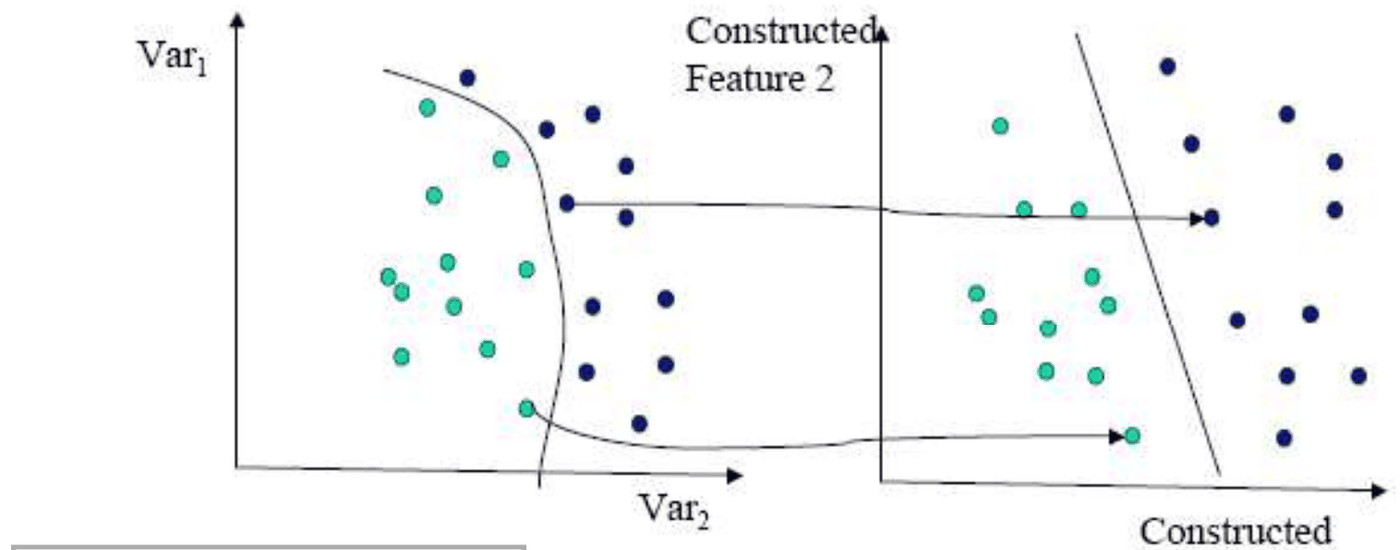
\includegraphics[width=0.91\linewidth,height=0.42\textheight,keepaspectratio]{images/13-svm_mapping.png}
\caption{Una funzione \(\Phi(\mathbf{x})\) mappa i dati in uno spazio in cui sono
linearmente separabili (si ricordi la LBE dei modelli lineari).}
\end{figure}

\begin{boxexample}{Da \(\mathbb{R}^2\) a \(\mathbb{R}^3\)}

Con \(\Phi: \mathbb{R}^2 \to \mathbb{R}^3\),
\((x_1, x_2)^T \mapsto (x_1^2, \sqrt{2}x_1x_2, x_2^2)^T\) (monomi di
secondo grado), due classi separate da un'ellisse nello spazio di input
diventano separabili da un \textbf{piano} nello spazio delle feature.

\end{boxexample}

\begin{figure}[htbp]
\centering
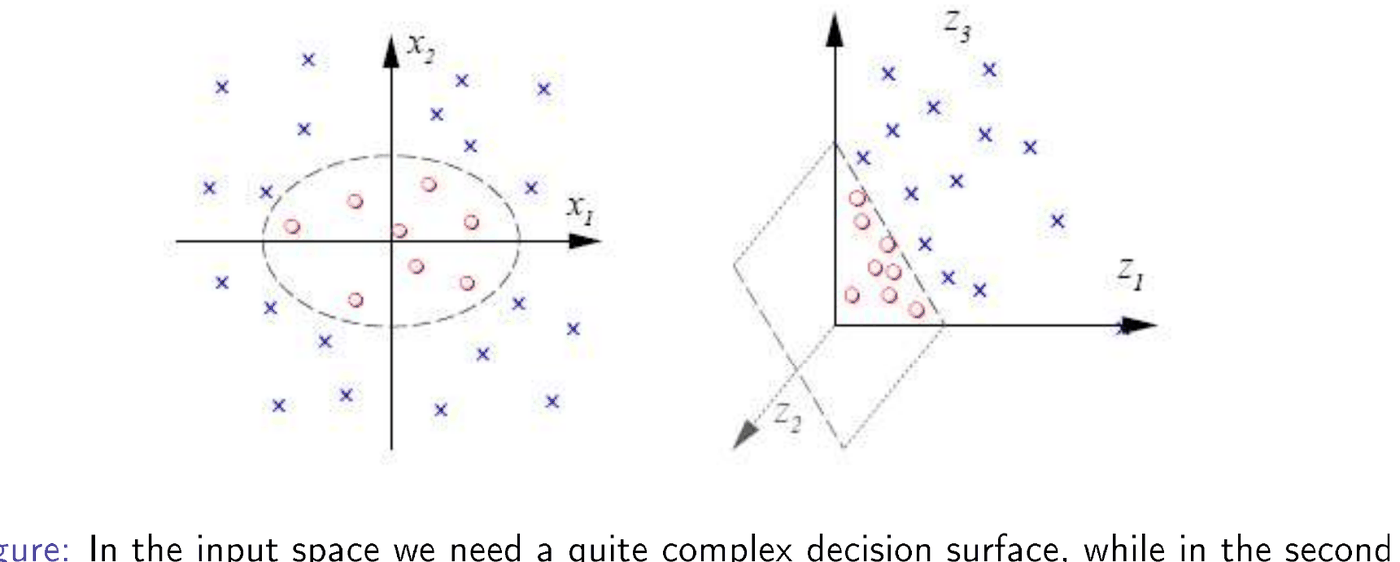
\includegraphics[width=0.89\linewidth,height=0.42\textheight,keepaspectratio]{images/13-svm_esempio-phi.png}
\caption{Nello spazio di input serve una superficie complessa; nello spazio dei
monomi di secondo grado basta una funzione lineare.}
\end{figure}

La mappatura dell'esempio è costruita apposta per risolvere il problema
(le feature corrispondono a ellissoidi nello spazio originale). Ma
trovare la trasformazione ``migliore'' \textbf{non è automatico} (a meno
di avere conoscenza a priori); spesso si usano trasformazioni generali.
\textbf{La scelta di \(\Phi\) è il punto critico delle SVM.}

\subsection{Spazi di feature ad alta
dimensione}\label{spazi-di-feature-ad-alta-dimensione}

Il procedimento è: (1) mappatura non lineare dei pattern in uno spazio
delle feature ad alta dimensione (per il \textbf{teorema di Cover}, i
pattern vi sono linearmente separabili con alta probabilità); (2)
ricerca dell'iperpiano ottimo nello spazio delle feature.

Ma sappiamo che spazi delle feature molto grandi (espansioni in basi
ampie) possono essere \textbf{computazionalmente infattibili} e portare
a \textbf{overfitting} senza controllare la dimensione dello spazio e la
complessità del classificatore. L'\textbf{approccio kernel} permette di
gestire lo spazio delle feature \textbf{implicitamente}, in un contesto
regolarizzato (dove è il \textbf{margine} a regolare la complessità, non
la dimensione dello spazio di input).

Con \(\Phi: \mathbb{R}^{m_0} \to \mathbb{R}^{m_1}\), il training set
diventa \(\{(\Phi(\mathbf{x}_i), d_i)\}\) e l'iperpiano
\(\mathbf{w}^T\Phi(\mathbf{x}) + b = 0\). Includendo il bias
(\(w_0 = b\), \(\phi_0(\mathbf{x}) = 1\)), la superficie di decisione
\(\mathbf{w}^T\Phi(\mathbf{x}) = 0\) è un'\textbf{espansione lineare in
basi} in cui la dimensione dello spazio può essere molto grande e la
complessità dipende dal \textbf{margine}, non dalla dimensione.

Il vettore dei pesi è
\(\mathbf{w} = \sum_i \alpha_i d_i\Phi(\mathbf{x}_i)\), e l'iperpiano
diventa \[
\sum_{i=1}^{N}\alpha_i d_i\,\underbrace{\Phi^T(\mathbf{x}_i)\Phi(\mathbf{x})}_{\text{prodotto scalare}} = 0.
\] Il prodotto scalare è ora nello spazio delle feature, e calcolare
\(\Phi(\mathbf{x})\) potrebbe essere intrattabile.

\subsection{Il kernel trick}\label{il-kernel-trick}

Sotto certe condizioni \textbf{non serve calcolare
\(\Phi(\mathbf{x})\)}, e nemmeno conoscere lo spazio delle feature!
Basta una funzione che calcoli direttamente il prodotto scalare nello
spazio delle feature:

\begin{boxdefinition}{Kernel (inner product kernel)}

\[
k: \mathbb{R}^{m_0} \times \mathbb{R}^{m_0} \to \mathbb{R}, \qquad k(\mathbf{x}_i, \mathbf{x}) = \Phi^T(\mathbf{x}_i)\,\Phi(\mathbf{x}).
\] Proprietà: è \textbf{simmetrica},
\(k(\mathbf{x}_i, \mathbf{x}) = k(\mathbf{x}, \mathbf{x}_i)\).

\end{boxdefinition}

\begin{boxexample}{Il kernel dell'esempio}

Con \(\Phi(\mathbf{x}) = (x_1^2, \sqrt{2}x_1x_2, x_2^2)^T\), per
\(\mathbf{x} = (x_1, x_2)^T\) e \(\mathbf{y} = (y_1, y_2)^T\): \[
\Phi^T(\mathbf{x})\Phi(\mathbf{y}) = x_1^2y_1^2 + 2x_1x_2y_1y_2 + x_2^2y_2^2 = (x_1y_1 + x_2y_2)^2 = (\mathbf{x}^T\mathbf{y})^2 = k(\mathbf{x}, \mathbf{y}).
\] \textbf{Molto importante}: il prodotto scalare nello spazio delle
feature (3D) viene calcolato \textbf{senza passare per la mappatura},
direttamente in termini dei pattern di input (2D).

\end{boxexample}

\subsection{La matrice kernel}\label{la-matrice-kernel}

I prodotti scalari tra le immagini dei pattern di training si
organizzano in una matrice \(N \times N\), la \textbf{matrice kernel} (o
matrice di Gram): \[
K = \{k(\mathbf{x}_i, \mathbf{x}_j)\}_{i,j=1}^N,
\] simmetrica perché il kernel è simmetrico.

\textbf{Ogni funzione kernel calcola un prodotto scalare in qualche
spazio?} No: la proprietà vale solo per i kernel che producono matrici
kernel \textbf{semidefinite positive} (\textbf{teorema di Mercer}), cioè
con autovalori non negativi.

Proprietà di chiusura: se \(k_1\) e \(k_2\) sono kernel, lo sono anche
\(k_1 + k_2\), \(\alpha k_1\) (con \(\alpha > 0\)) e \(k_1 k_2\).

\subsection{SVM con kernel}\label{svm-con-kernel}

Il primale nello spazio delle feature è lo stesso del soft margin con
\(\Phi(\mathbf{x}_i)\) al posto di \(\mathbf{x}_i\) (ma \(\mathbf{w}\)
vive nello spazio delle feature, che può rendere il problema
intrattabile). Il \textbf{duale} invece è trattabile:

\begin{boxdefinition}{Problema duale nello spazio delle feature}

Trovare \(\{\alpha_i\}\) che massimizzano \[
Q(\boldsymbol{\alpha}) = \sum_{i=1}^{N}\alpha_i - \frac{1}{2}\sum_{i,j=1}^{N}\alpha_i\alpha_j d_i d_j\,\underbrace{k(\mathbf{x}_i, \mathbf{x}_j)}_{K_{ij}}
\] soggetto a \(\sum_i\alpha_i d_i = 0\) e \(0 \le \alpha_i \le C\).

\end{boxdefinition}

Il kernel incorpora la mappatura nello spazio delle feature. La
dipendenza da \(N\) (anziché dalla dimensione dello spazio) diventa ora
un \textbf{vantaggio}, perché lo spazio delle feature può avere
dimensione altissima o infinita.

\begin{boxabstract}{Riepilogo del procedimento}

\begin{enumerate}
\def\labelenumi{\arabic{enumi}.}
\tightlist
\item
  Si ha il training set \(T = \{(\mathbf{x}_i, d_i)\}\).
\item
  Si scelgono il parametro \(C\) e la funzione kernel \(k\).
\item
  Si calcola la matrice kernel \(K\).
\item
  Si risolve il problema di ottimizzazione (programmazione quadratica)
  trovando \(\{\alpha_i\}\).
\item
  Si calcola il bias \(b\) dai moltiplicatori e dalla matrice kernel.
\item
  Per un nuovo pattern \(\mathbf{x}\):
  \(\mathbf{w}^T\Phi(\mathbf{x}) = \sum_i\alpha_i d_i\,k(\mathbf{x}, \mathbf{x}_i) + b\)
  (senza mai calcolare \(\mathbf{w}\)!), e si classifica con il segno.
\end{enumerate}

\textbf{Sparsità}: la soluzione è sparsa negli \(\alpha\), perché tutti
i moltiplicatori dei non-support vector sono nulli.

\end{boxabstract}

In fase di test:
\(h(\mathbf{x}) = \operatorname{sign}\left(\sum_i\alpha_i d_i\,k(\mathbf{x}, \mathbf{x}_i) + b\right)\).
Si memorizzano gli \(\mathbf{x}_i\) (i support vector) per la fase di
test: somiglia al K-NN?

\subsection{Vista ``architetturale'' di una
SVM}\label{vista-architetturale-di-una-svm}

\begin{figure}[htbp]
\centering
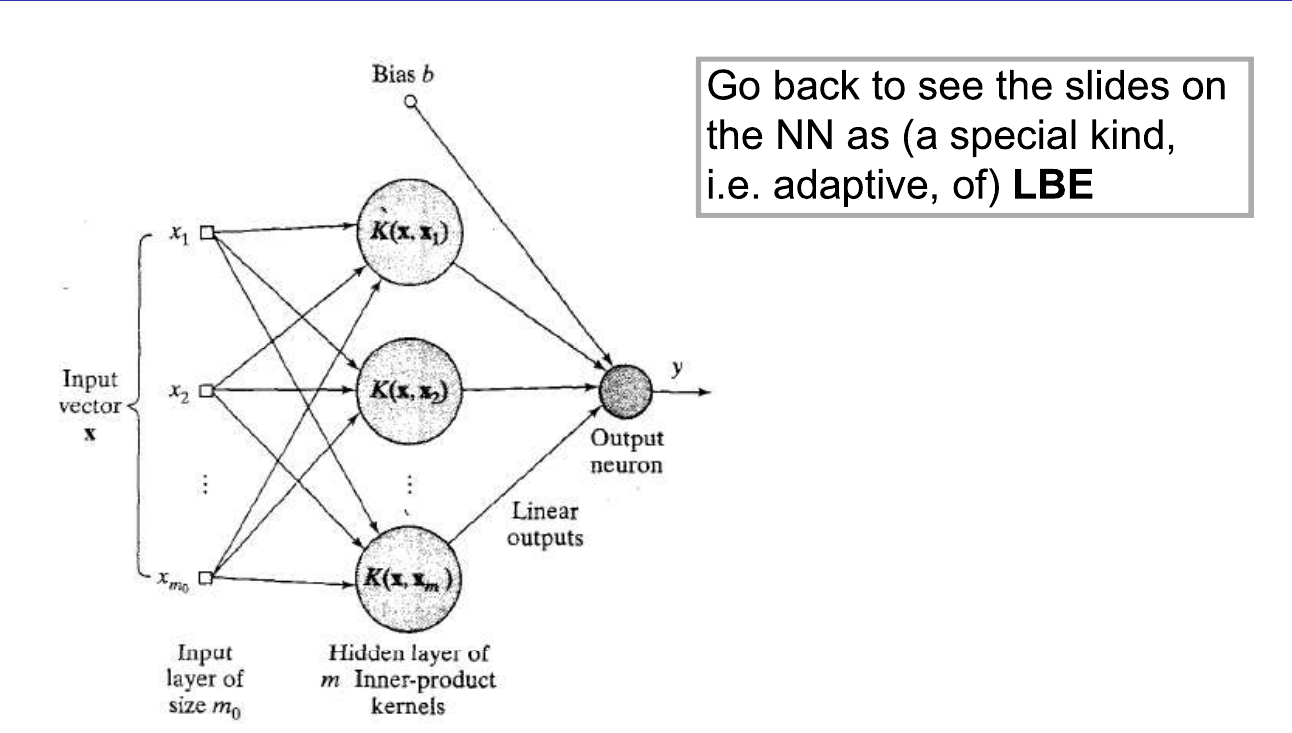
\includegraphics[width=0.66\linewidth,height=0.42\textheight,keepaspectratio]{images/13-svm_architettura.png}
\caption{``Architettura'' di una SVM: numero di unità nascoste = numero di
support vector.}
\end{figure}

Il numero di ``unità nascoste'' è pari al \textbf{numero di support
vector}, ma non sono esattamente le stesse unità di una rete neurale: le
unità nascoste di una rete hanno \textbf{parametri liberi adattivi}, qui
invece i ``centri'' sono i support vector stessi e la funzione è fissata
dal kernel. È solo una vista illustrativa: da confrontare con le reti
neurali (una forma adattiva di LBE) in termini di controllo della
complessità, efficienza e altre caratteristiche.

\subsection{Esempi di kernel}\label{esempi-di-kernel}

\begin{itemize}
\tightlist
\item
  \textbf{Polinomiale}:
  \(k(\mathbf{x}, \mathbf{x}_i) = (\mathbf{x}^T\mathbf{x}_i + 1)^p\),
  con \(p\) scelto dall'utente.
\item
  \textbf{RBF} (\emph{Radial Basis Function}, detto anche \textbf{kernel
  gaussiano}):
  \(k(\mathbf{x}, \mathbf{x}_i) = e^{-\frac{1}{2\sigma^2}\|\mathbf{x} - \mathbf{x}_i\|^2}\),
  con \(\sigma^2\) scelto dall'utente. Con kernel molto ``stretti''
  (\(\sigma\) piccolo) la risposta su \(\mathbf{x}_i\) è solo \(d_i\)
  (somiglia al 1-NN!).
\item
  \textbf{Perceptron a due strati}:
  \(k(\mathbf{x}, \mathbf{x}_i) = \tanh(\beta_0\mathbf{x}^T\mathbf{x}_i + \beta_1)\),
  con \(\beta_0 > 0\) e \(\beta_1 < 0\).
\end{itemize}

\begin{boxwarning}{Importante}

Per il kernel polinomiale e l'RBF si ottiene \textbf{sempre} un kernel
valido (prodotto scalare), mentre per il perceptron a due strati il
teorema di Mercer vale solo per alcune scelte di \(\beta_0\) e
\(\beta_1\). Un kernel RBF corrisponde sempre a uno spazio delle feature
di \textbf{dimensione infinita}.

\end{boxwarning}

\section{Parte II --- SVM per la regressione non
lineare}\label{parte-ii-svm-per-la-regressione-non-lineare}

\subsection{Il problema}\label{il-problema}

Si ha \(d = f(\mathbf{x}) + v\), con \(f\) sconosciuta e rumore \(v\)
indipendente da \(\mathbf{x}\). Si stima \(d\) con un'espansione lineare
di funzioni non lineari: \[
y = h(\mathbf{x}) = \mathbf{w}^T\Phi(\mathbf{x}), \qquad \mathbf{w} = (b, w_1, \dots, w_{m_1})^T, \quad \Phi(\mathbf{x}) = (1, \phi_1(\mathbf{x}), \dots, \phi_{m_1}(\mathbf{x}))^T.
\]

\subsection{\texorpdfstring{La loss
\(\varepsilon\)-insensitive}{La loss \textbackslash varepsilon-insensitive}}\label{la-loss-varepsilon-insensitive}

\[
L_\varepsilon(d, y) = \begin{cases} |d - y| - \varepsilon & \text{se } |d - y| \ge \varepsilon \\ 0 & \text{altrimenti.} \end{cases}
\]

\begin{figure}[htbp]
\centering
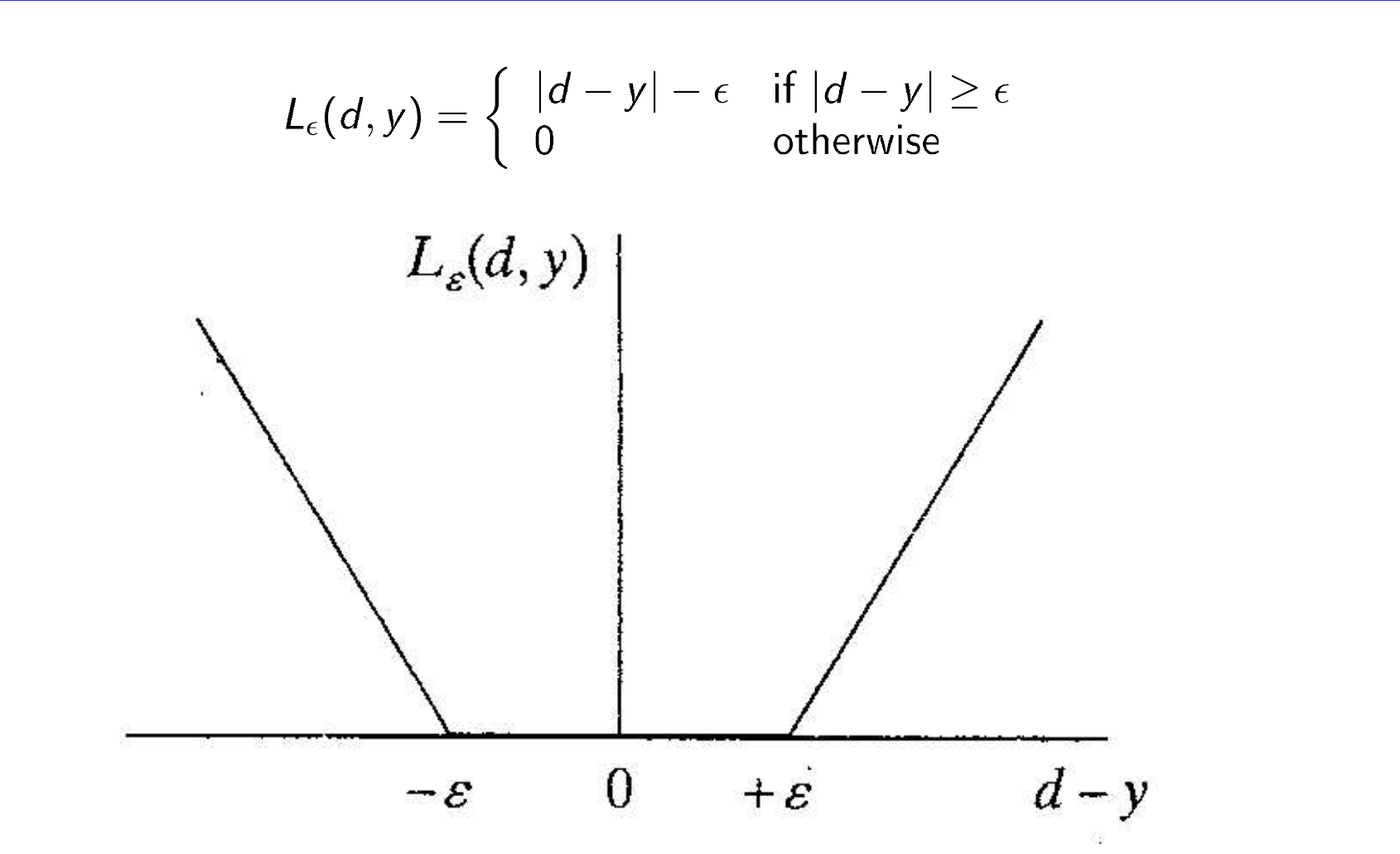
\includegraphics[width=0.54\linewidth,height=0.42\textheight,keepaspectratio]{images/13-svm_eps-loss.png}
\caption{La loss \(\varepsilon\)-insensitive (o}
\end{figure}

Gli errori più piccoli di \(\varepsilon\) \textbf{non costano nulla}: si
forma un \textbf{tubo} di ampiezza \(\varepsilon\) attorno alla
predizione, e solo i punti fuori dal tubo contribuiscono alla loss. Di
nuovo, \textbf{solo i support vector guidano la soluzione}: nella
classificazione erano i punti oltre il margine, qui sono i punti fuori
dal tubo.

\begin{figure}[htbp]
\centering
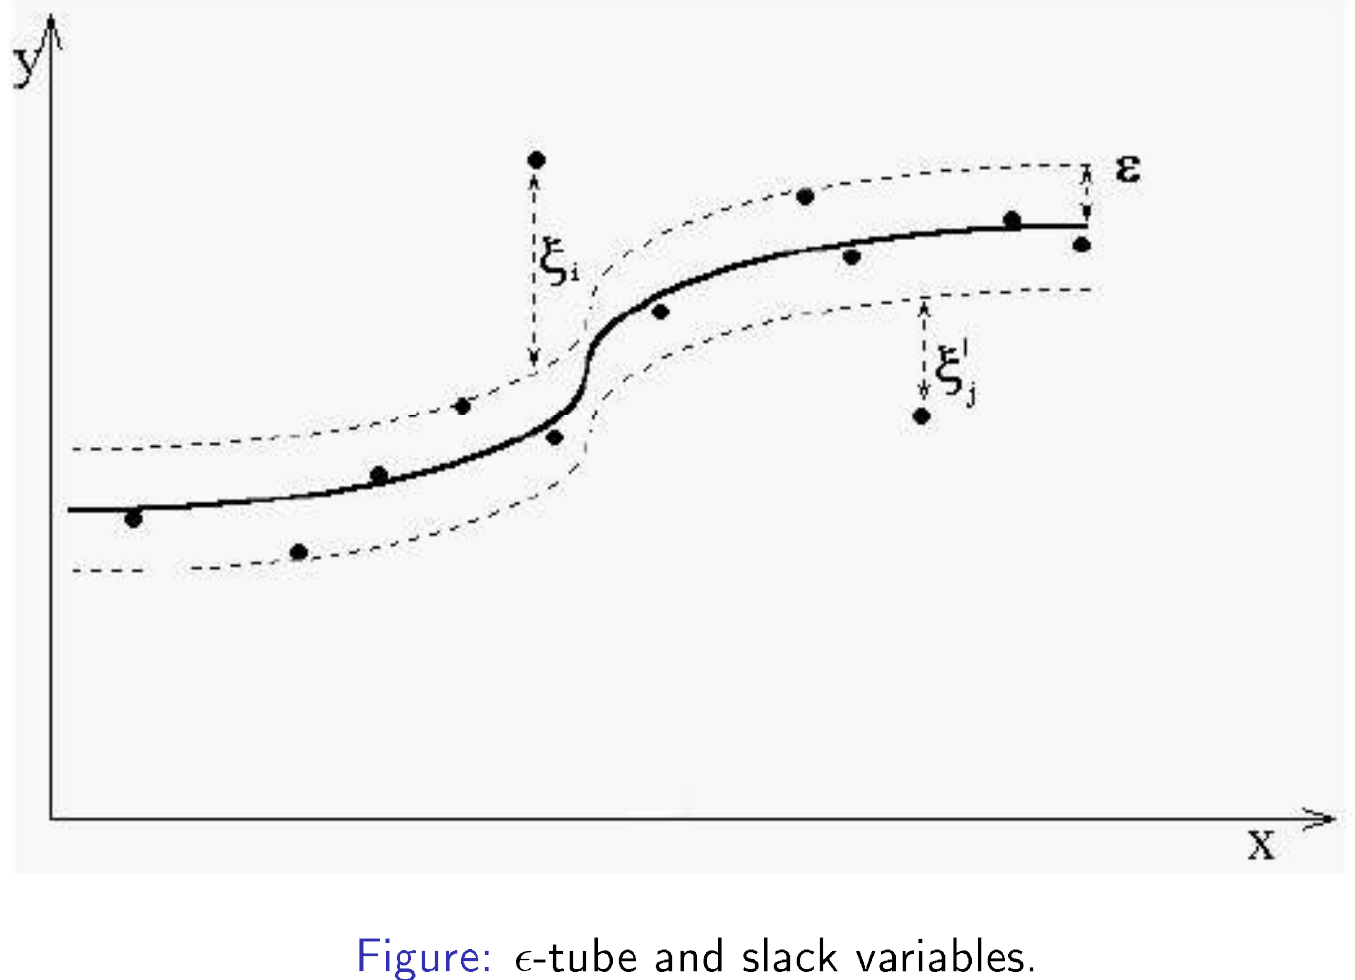
\includegraphics[width=0.60\linewidth,height=0.42\textheight,keepaspectratio]{images/13-svm_eps-tube.png}
\caption{Il tubo \(\varepsilon\) e le variabili slack per la regressione.}
\end{figure}

\subsection{Formulazione}\label{formulazione}

Si introducono due insiemi di variabili slack non negative \(\xi_i\) e
\(\xi'_i\) (sopra e sotto il tubo): \[
-\xi'_i - \varepsilon \le d_i - \mathbf{w}^T\Phi(\mathbf{x}_i) \le \varepsilon + \xi_i.
\]

\begin{boxdefinition}{Problema primale --- SVM per la regressione}

Minimizzare \[
\Psi(\mathbf{w}, \boldsymbol{\xi}, \boldsymbol{\xi}') = \frac{1}{2}\mathbf{w}^T\mathbf{w} + C\sum_{i=1}^{N}(\xi_i + \xi'_i)
\] soggetto a
\(d_i - \mathbf{w}^T\Phi(\mathbf{x}_i) \le \varepsilon + \xi_i\),
\(\;\mathbf{w}^T\Phi(\mathbf{x}_i) - d_i \le \varepsilon + \xi'_i\),
\(\;\xi_i \ge 0\), \(\;\xi'_i \ge 0\).

\end{boxdefinition}

\begin{boxdefinition}{Problema duale --- SVM per la regressione*}

Trovare \(\{\alpha_i\}\) e \(\{\alpha'_i\}\) che massimizzano \[
Q(\boldsymbol{\alpha}, \boldsymbol{\alpha}') = \sum_{i=1}^{N}d_i(\alpha_i - \alpha'_i) - \varepsilon\sum_{i=1}^{N}(\alpha_i + \alpha'_i) - \frac{1}{2}\sum_{i,j=1}^{N}(\alpha_i - \alpha'_i)(\alpha_j - \alpha'_j)\,k(\mathbf{x}_i, \mathbf{x}_j)
\] soggetto a \(\sum_i(\alpha_i - \alpha'_i) = 0\) e
\(0 \le \alpha_i, \alpha'_i \le C\).

\end{boxdefinition}

Dalla soluzione: \[
\mathbf{w} = \sum_{i=1}^{N}\underbrace{(\alpha_i - \alpha'_i)}_{\gamma_i}\Phi(\mathbf{x}_i), \qquad h(\mathbf{x}) = \sum_{i=1}^{N}\gamma_i\,\Phi^T(\mathbf{x}_i)\Phi(\mathbf{x}) = \sum_{i=1}^{N}\gamma_i\,k(\mathbf{x}_i, \mathbf{x}).
\] I \textbf{support vector} corrispondono ai \(\gamma_i\) non nulli.

\begin{boxabstract}{Riepilogo per la regressione}

\begin{enumerate}
\def\labelenumi{\arabic{enumi}.}
\tightlist
\item
  Scegliere i parametri \(C\) ed \(\varepsilon\).
\item
  Scegliere un kernel \(k\).
\item
  Calcolare la matrice kernel \(K\).
\item
  Risolvere il duale e ottenere i \(\gamma_i\).
\item
  Calcolare il bias ottimo.
\item
  La funzione stimata è una combinazione lineare di prodotti scalari in
  uno spazio delle feature che possiamo ignorare:
  \(h(\mathbf{x}) = \sum_i\gamma_i\,k(\mathbf{x}_i, \mathbf{x})\).
\end{enumerate}

\end{boxabstract}

\begin{boxquestion}{Cosa bisogna sapere}

\begin{itemize}
\tightlist
\item
  La definizione di classificatore a \textbf{margine massimo}.
\item
  Come il margine massimo si trasforma in un problema di
  \textbf{programmazione quadratica}.
\item
  Cosa la QP fa per noi (non come lo fa).
\item
  Perché l'SVM approssima la \textbf{SRM}.
\item
  Come si gestiscono dati \textbf{rumorosi} (non separabili): soft
  margin.
\item
  Come si ottengono \textbf{confini non lineari}: kernel.
\item
  Come i kernel permettono di lavorare con espansioni in basi di
  dimensione altissima senza calcolarle.
\item
  Come funziona la SVM per la regressione (\(\varepsilon\)-insensitive
  loss).
\end{itemize}

\end{boxquestion}

Riferimenti: Haykin, \emph{Neural Networks} (2ª ed.), cap. 6
(``necessario e sufficiente''); Burges, \emph{A Tutorial on Support
Vector Machines for Pattern Recognition}; Schölkopf e Smola,
\emph{Learning with Kernels}; Vapnik, \emph{The Nature of Statistical
Learning Theory} e \emph{An Overview of Statistical Learning Theory}
(1999).
